\documentclass[tikz,border=10pt]{standalone}
\usepackage{tikz}
\definecolor{bgpage}{HTML}{171D2B}
\definecolor{aksen}{HTML}{F7B538}
\pagecolor{bgpage}

\begin{document}
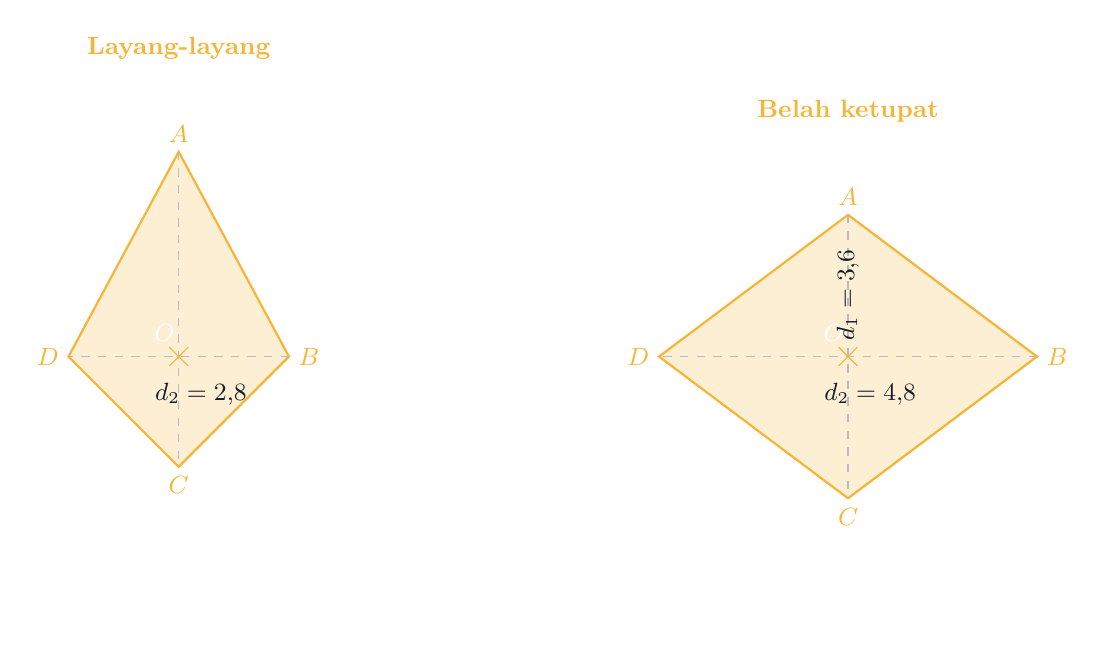
\begin{tikzpicture}[
  scale=1.0,
  every node/.style={text=white, font=\small},
  bangun/.style={thick, draw=aksen, fill=aksen!22},
  diag/.style={dashed, draw=white!70!bgpage},
  lab/.style={text=white, font=\small},
  darl/.style={text=bgpage, font=\small},
  labk/.style={text=aksen, font=\small\bfseries},
]

% ---------- Layang-layang (kiri) ----------
\begin{scope}[xshift=0cm]
  \coordinate (O) at (0,0);
  \coordinate (A) at (0,2.6);
  \coordinate (B) at (1.4,0);
  \coordinate (C) at (0,-1.4);
  \coordinate (D) at (-1.4,0);
  
  \draw[bangun] (A) -- (B) -- (C) -- (D) -- cycle;
  \draw[diag] (A) -- (C);
  \draw[diag] (B) -- (D);
  \draw[aksen] (-0.12,0.12) -- (0.12,-0.12) (-0.12,-0.12) -- (0.12,0.12);
  \node[labk, above] at (A) {$A$};
  \node[labk, right] at (B) {$B$};
  \node[labk, below] at (C) {$C$};
  \node[labk, left]  at (D) {$D$};
  \node[lab, above left, xshift=2pt, yshift=2pt] at (O) {$O$};
  \node[lab, rotate=0, right, xshift=10pt, yshift=-6pt] at (0.35,1.75) {$d_1 = 4{,}0$};
  \node[darl, below, xshift=8pt, yshift=-6pt] at (0,0) {$d_2 = 2{,}8$};
  \node[lab, right, xshift=4pt] at (0.7,1.3) {$s_1$};
  \node[lab, left, xshift=-4pt] at (-0.7,1.3) {$s_1$};
  \node[lab, right, xshift=4pt] at (0.7,-0.7) {$s_2$};
  \node[lab, left, xshift=-4pt] at (-0.7,-0.7) {$s_2$};
  \node[labk, font=\small\bfseries, above, yshift=30pt] at (0,2.6) {Layang-layang};
  \node[lab, below, yshift=-30pt] at (0,-1.4) {$OA \neq OC$, \ $OB = OD$};
\end{scope}

% ---------- Belah ketupat (kanan) ----------
\begin{scope}[xshift=8.5cm]
  \coordinate (O) at (0,0);
  \coordinate (A) at (0,1.8);
  \coordinate (B) at (2.4,0);
  \coordinate (C) at (0,-1.8);
  \coordinate (D) at (-2.4,0);
  
  \draw[bangun] (A) -- (B) -- (C) -- (D) -- cycle;
  \draw[diag] (A) -- (C);
  \draw[diag] (B) -- (D);
  \draw[aksen] (-0.12,0.12) -- (0.12,-0.12) (-0.12,-0.12) -- (0.12,0.12);
  \node[labk, above] at (A) {$A$};
  \node[labk, right] at (B) {$B$};
  \node[labk, below] at (C) {$C$};
  \node[labk, left]  at (D) {$D$};
  \node[lab, above left, xshift=2pt, yshift=2pt] at (O) {$O$};
  \node[darl, rotate=90, xshift=8pt] at (0,0.5) {$d_1 = 3{,}6$};
  \node[darl, below, xshift=8pt, yshift=-6pt] at (0,0) {$d_2 = 4{,}8$};
  \node[labk, font=\small\bfseries, above, yshift=30pt] at (0,1.8) {Belah ketupat};
  \node[lab, below, yshift=-30pt] at (0,-1.8) {$OA = OC$, \ $OB = OD$};
\end{scope}

\end{tikzpicture}
\end{document}
